% Manuscript for IEEE Transactions on Instrumentation and Measurement.
% Build: latexmk -pdf main.tex   (or `make paper` from the repository root)
% Figures: python scripts/paper_figures.py   (reads results/, writes manuscript/figures/)
\documentclass[lettersize,journal]{IEEEtran}
\usepackage{amsmath,amsfonts}
\usepackage{array}
\usepackage{booktabs}
\usepackage{textcomp}
\usepackage{stfloats}
\usepackage{url}
\usepackage{graphicx}
\usepackage{cite}
\usepackage{siunitx}
\usepackage{xcolor}
\graphicspath{{figures/}}
% units in math mode (the text font has no upright omega); bold and italic context is kept
\sisetup{range-phrase={--}, range-units=single, per-mode=symbol,
  reset-text-series=false, text-series-to-math=true,
  reset-text-shape=false, reset-text-family=false}
\hyphenation{elec-trode elec-trodes meas-ure-ment meas-ure-ments}

% Anything still to be supplied or confirmed by the authors. Search for \todo before submission.
\newcommand{\todo}[1]{\textcolor{red}{[TODO: #1]}}
\newcommand{\cA}{Circuit~A}
\newcommand{\cB}{Circuit~B}

\begin{document}

\title{Specification-Aware Fault Diagnosis of ECG Analog Front-Ends: Bridging Alternate Test and
Machine-Learning Diagnosis for In-Service Self-Test}

\author{Telmo~Miguel-Medina%
\thanks{Manuscript received October 4, 2026.}%
\thanks{T. Miguel-Medina is with the Electromechanical Engineering Department, University of
Burgos, Burgos, Spain (e-mail: tmiguel@ubu.es; ORCID: 0009-0004-0654-6650).}%
\thanks{This article has supplementary material provided by the author. The dataset and the code
are openly available; see the Data and Code Availability section.}}

\markboth{IEEE Transactions on Instrumentation and Measurement}%
{Miguel-Medina: Specification-Aware Fault Diagnosis of ECG Analog Front-Ends}

\maketitle

\begin{abstract}
An electrocardiograph whose analog front-end has drifted out of specification still produces a
trace. This paper studies, by simulation, a self-test that the instrument can run in service with its own converter and
internal test signals. Two questions that the literature treats separately are joined: whether
the circuit still complies with the requirements of IEC~60601-2-25, as in alternate test, and
which component is responsible, as in machine-learning fault diagnosis. A third one is added:
whether the cause lies in the circuit or in the electrodes. About \num{130000} Monte Carlo cases
of two front-ends (an integrated instrumentation amplifier with its discrete network, and a
discrete three-op-amp amplifier) are simulated with hard, parametric and electrode faults, gel
and dry electrodes, and eleven specification values per case. On the integrated design a
classifier reaches \SI{0.9}{\percent} of escapes at \SI{7.8}{\percent} of false rejects, against
\SI{22.5}{\percent} and \SI{20.0}{\percent} for a limit test. Labeling a fault by component
deviation instead of by loss of compliance raises false rejects from \SI{1.6}{\percent} to
\SI{37}{\percent}. The groups of components that cannot be told apart are predicted from the
sensitivities of the nominal circuit; diagnosis at that level reaches a macro F1 of 0.87 and
holds for fault magnitudes absent from training, whereas component-level diagnosis does not.
Non-compliant circuits are recognized in \SI{94}{\percent} of the cases and electrode problems in
\SI{64}{\percent}. Three measurements taking \SI{3}{\second} decide compliance within one point
of the balanced accuracy of the complete \SI{97}{\second} self-test.
\end{abstract}

\begin{IEEEkeywords}
Alternate test, ambiguity groups, analog fault diagnosis, biopotential amplifier, built-in
self-test, electrocardiography, machine learning, skin-electrode impedance.
\end{IEEEkeywords}

\section{Introduction}
\IEEEPARstart{A}{n} electrocardiograph that has drifted out of specification still produces a
trace. A gain error of ten percent, a low-frequency corner that has moved, or a degraded
common-mode rejection do not stop the instrument; they change the amplitudes and the ST segment
that a clinician or an algorithm will read. The required performance is laid down in
IEC~60601-2-25~\cite{iec60601225}, but conformance is verified with external equipment, at type
testing and at periodic maintenance. In between, the instrument cannot know whether its analog
front-end still complies, and the deviations that appear in use are precisely those that the user
lacks the equipment to detect~\cite{chen2025}.

What the instrument can do on its own is limited. Integrated front-ends detect a detached
electrode and provide internal test signals to verify the signal chain at power-up; these are
applied inside the device and, by the manufacturer's own account, are not intended for compliance
testing~\cite{ads1298}. They do not cover the discrete network around the amplifier (protection
and bias resistors, gain-setting resistor, coupling and anti-aliasing filters, driven-right-leg
network, reference divider), nor say whether a deviation matters.

Two research communities have worked on parts of this problem without meeting. The analog test
community checks conformance to specifications, and alternate test replaces direct specification
measurements by cheap signatures from which pass or fail is inferred, with the explicit aim of
neither accepting a bad circuit nor rejecting a good
one~\cite{cheng2010,variyam1998spec,variyam1998synth,voorakaranam2007}; it targets production
test of integrated circuits. The fault-diagnosis community asks which component has failed and
answers with classifiers trained on simulated
faults~\cite{dieste2021,dieste2024,dieste2025,yang2020,rajpal2026}; there a fault is a component
that deviates from nominal by a fixed percentage, and whether the circuit is still within
specification is not asked.

For a medical instrument both questions matter, and a third appears: whether the problem is in
the circuit at all, since the skin-electrode interface is part of the signal path and varies by
orders of magnitude between subjects and electrode types~\cite{joutsen2024}. A percentage
definition of a fault is of little use here: in the front-ends studied in this paper, more than
\SI{93}{\percent} of the circuits with one component \SI{5}{\percent} off nominal, and more than
half of those with one component \SI{50}{\percent} off, still meet every requirement of the
standard. The circuit is a further issue. Chen \emph{et al.}~\cite{chen2025} have shown that the
symmetries of the usual benchmark circuits make different faults indistinguishable, and they
redesign the training circuit to remove them. An instrument designer cannot: the circuit is
given. What can be done is to find out in advance which components are indistinguishable and
report the diagnosis at that level.

This paper studies, by simulation, an in-service self-test of a single-lead ECG front-end that
uses only what the instrument can acquire with its own converter and internal test signals. Two
circuits are considered: a realistic one built around an integrated instrumentation amplifier
(\cA) and a discrete three-op-amp amplifier that stands for the circuits of the diagnosis
literature (\cB). The contributions are as follows.
\begin{enumerate}
\item A two-level self-test that joins specification verification and fault location for a
discrete front-end network. On \cA, compliance with IEC~60601-2-25 is decided with
\SI{0.9}{\percent} of escapes at \SI{7.8}{\percent} of false rejects, where a limit test on the
same measurements gives \SI{22.5}{\percent} and \SI{20.0}{\percent}.
\item A simulation study with manufacturing tolerances of a biopotential front-end of realistic
architecture: about \num{130000} Monte Carlo cases with hard, parametric, amplifier and electrode
faults, each labeled with eleven clinical specifications.
\item The separation of electrode problems from circuit faults, with gel and measured dry
electrodes~\cite{iec60601225,joutsen2024}, and the identification of its physical limit.
\item A quantified comparison of functional and percentage severity: training on component
deviation instead of on compliance raises false rejects from \SI{1.6}{\percent} to
\SI{37}{\percent}.
\item An open dataset and code.
\end{enumerate}
In addition, the groups of components that cannot be told apart are obtained from the
sensitivities of the nominal circuit, before any fault is simulated, and they explain why
component-level diagnosis does not generalize to unseen fault magnitudes while group-level
diagnosis does.

The study is based on simulation only, for two reasons. Labeling a case requires the eleven
tests of the standard, and the campaign covers some 600 fault conditions with 200 realizations
each, most of which require a component to be altered; neither is feasible on hardware at that
scale. And which faults break compliance, which can be seen and which can be told apart has to
be known before a bench experiment on a meaningful subset can be designed. Validation on hardware
is the next step.

\section{Related Work}
\label{sec:related}

\subsubsection*{Machine-learning diagnosis}
Typical studies simulate hard or soft faults under component tolerances, extract features from
node voltages or from the frequency or time response, and train a classifier. Dieste-Velasco has
addressed hard faults in transistor amplifier stages with a neural network on a few accessible
measurements, after grouping the faults that those measurements cannot tell
apart~\cite{dieste2021}; hard faults with a fuzzy inference system~\cite{dieste2024}; and soft
faults in a Sallen-Key band-pass filter with seven classifiers on six voltages, reaching a
classification accuracy of \SI{97.9}{\percent} over fifteen classes~\cite{dieste2025}. Deep
models on raw responses~\cite{yang2020} and explainable classifiers on frequency-response
features~\cite{rajpal2026} are also used. Three aspects matter here. The Sallen-Key band-pass and
the four-op-amp biquad high-pass filters recur as
benchmarks~\cite{dieste2025,chen2025,zhang2026,srimani2022}, and their symmetries produce
overlapping fault responses~\cite{chen2025}. Generalization across fault severities is an open
problem: transferring from a \SI{50}{\percent} to a \SI{25}{\percent} deviation with diffusion
augmentation and domain adaptation reaches \SI{71}{\percent} on thirteen classes, a figure its
authors present as an upper bound~\cite{zhang2026}. And testability theory defines ambiguity
groups as sets of components whose faults cannot be distinguished from the available
measurements~\cite{starzyk2000}. In all this work a fault is a deviation of a component, usually
25 or \SI{50}{\percent} against tolerances of 5 to \SI{10}{\percent}; whether the circuit still
meets its requirements is not considered.

\subsubsection*{Specification-based and alternate test}
Alternate test predicts the specifications, or directly the pass/fail outcome, from signatures
that are cheap to measure; the acceptance region in signature space comes from Monte Carlo
simulation and statistical classification, or a regression from signatures to specifications is
calibrated on measured devices~\cite{cheng2010,voorakaranam2007}. Variyam and Chatterjee
formulated test generation as the reduction of the probability of misclassifying a bad circuit as
good and vice versa~\cite{variyam1998spec,variyam1998synth}, and redundant specification tests
can be removed by statistical learning~\cite{biswas2005}. Alternate test has also served
diagnosis: signatures from built-in sensors are related by statistical learning to the source of
a failure in integrated RF transceivers~\cite{cheng2010}. Our work follows that principle with a
different object and setting: the components of a discrete network instead of the blocks of an
integrated circuit, a self-test in service with the instrument's own converter instead of
production test, the requirements of a clinical standard instead of data-sheet specifications,
and a confounder, the electrode, with no counterpart in integrated-circuit test.

\subsubsection*{Biomedical equipment and electrodes}
Work on faults in ECG acquisition operates on the recorded signal and detects that the data are
bad~\cite{agarwal2022,khezripour2026,adams2026}, not which part of the circuit has failed nor
whether the instrument still complies. At circuit level we have found two precedents: faults of a
simulated electroencephalograph circuit classified with wavelet features and a neural network,
without a description of circuit or faults~\cite{gao2025}, and board-level diagnosis of a therapy
device from port signals and symptoms~\cite{liu2021}. Neither considers tolerances,
specifications or electrodes. The standard represents the skin-electrode impedance by
\SI{51}{\kilo\ohm} in parallel with \SI{47}{\nano\farad}~\cite{iec60601225}, whereas dry
electrodes range from about \SI{0.1}{\mega\ohm} to almost \SI{9}{\mega\ohm}, with differences of
one to three orders of magnitude between subjects~\cite{joutsen2024}. Such an impedance forms a
divider with the input network, so a healthy instrument on a high-impedance electrode can
resemble a faulty one on a good electrode, and any imbalance converts common-mode interference
into a differential signal that the driven-right-leg circuit reduces but does not
cancel~\cite{winter1983}. To our knowledge no previous work separates electrode degradation from
a fault of the circuit behind it.

\section{Methods}
\label{sec:methods}

Every simulated case is one realization of a front-end: its components drawn within
manufacturing tolerances, at most one injected fault, and three electrodes drawn from a
population. Two simulations are run per case. The first takes the measurements that the
instrument could take on itself, with the patient's electrodes connected, and gives the
features. The second measures the specifications with the test networks of the standard and
gives the labels.

\subsection{Circuits}
\label{sec:circuits}

\begin{figure*}[!t]
\centering
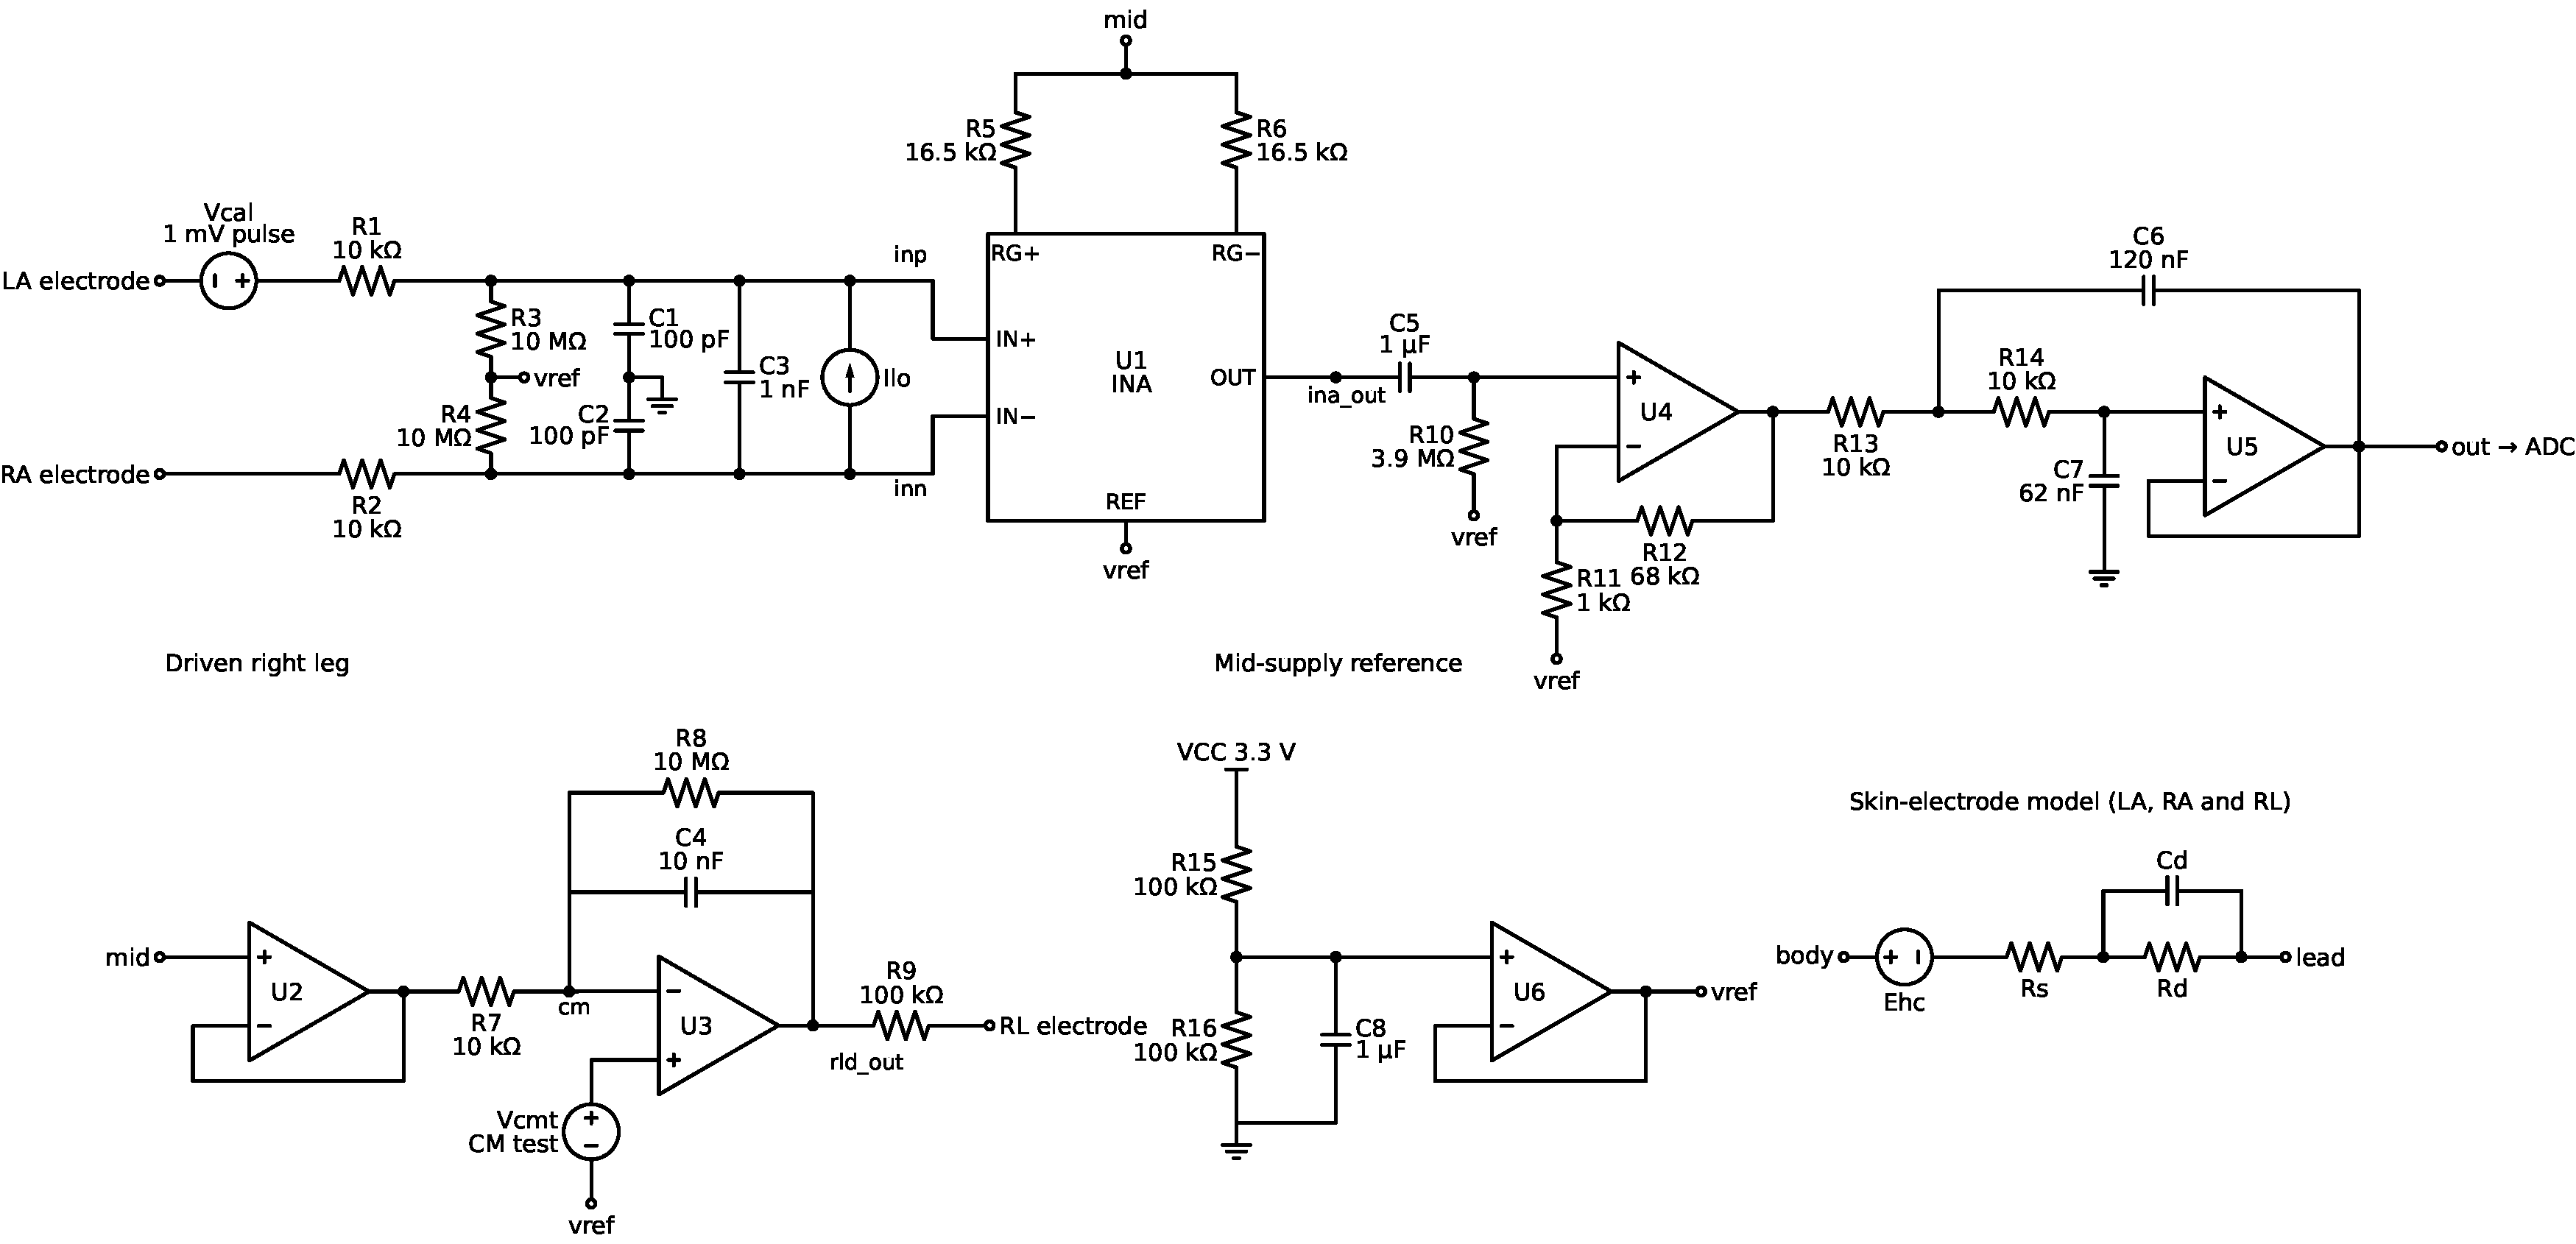
\includegraphics[width=\textwidth]{schematic_integrated}
\caption{\cA: integrated instrumentation amplifier with its discrete network, on a single
\SI{3.3}{\volt} supply. $V_\mathrm{cal}$, $V_\mathrm{cmt}$ and $I_\mathrm{lo}$ are the internal
self-test sources; nets with the same name are connected. The electrode model at the lower right
is placed between the body and each of the three leads.}
\label{fig:schematic}
\end{figure*}

Both circuits are single-lead front-ends with the same chain: input protection and
radio-frequency filtering, bias resistors, an instrumentation amplifier, a first-order high-pass
filter, a gain stage, a Sallen-Key low-pass filter and a driven-right-leg (DRL) integrator.

\cA\ (Fig.~\ref{fig:schematic}) is built around a Texas Instruments INA333~\cite{ina333} on a
single \SI{3.3}{\volt} supply; it has 16 resistors, 8 capacitors and 5 discrete op-amps, and a
gain of 278. Its values follow from the standard: a first-stage gain of 4.03 keeps a
$\pm$\SI{300}{\milli\volt} electrode offset within the output swing; the high-pass corner is
\SI{0.041}{\hertz}, as the impulse test requires; the low-pass filter is a Butterworth response
at \SI{185}{\hertz}. \cB\ replaces the integrated amplifier by three op-amps and seven resistors
on $\pm$\SI{5}{\volt} supplies (20 resistors, 6 capacitors, 6 op-amps, gain 414). It has the
resistor symmetries identified in benchmark circuits~\cite{chen2025}; its schematic is in the
supplementary material.

The circuits are simulated with ngspice~\cite{ngspice}. The INA333 is a behavioral model built
from its data sheet (three-amplifier structure, single pole, noise, output clamping, offset and
finite common-mode rejection ratio, CMRR), and the op-amps are single-pole models with offset,
noise and clamping. Against the manufacturer's macromodel of the amplifier alone, gain and CMRR
at \SI{50}{\hertz} agree (\SI{102}{\decibel} against \SI{100}{\decibel}); the macromodel was not
used because its fixed parameters allow neither Monte Carlo variation nor faults in the block.
Healthy variation draws resistors uniformly within $\pm$\SI{1}{\percent} and capacitors within
$\pm$\SI{5}{\percent}, and amplifier parameters within their data-sheet ranges.

\subsection{Electrodes}
\label{sec:electrodes}

Each electrode is a half-cell potential in series with $R_s$ and with $R_d \parallel C_d$. Half
of the cases use gel electrodes, with the network of the standard (\SI{51}{\kilo\ohm} in parallel
with \SI{47}{\nano\farad}). The other half use one of six dry materials (conductive polymer,
conductive fabric with and without a membrane, stainless steel, silver, platinum) with the
parameters fitted in~\cite{joutsen2024}; for each case one of the six subjects of the open data
of that work is drawn and that subject's contact resistance is used, which spans
\SI{0.26}{\mega\ohm} to \SI{68}{\mega\ohm} for the polymer and the fabrics (referred to below as
porous electrodes) and \SI{0.6}{\kilo\ohm} to \SI{0.58}{\mega\ohm} for the solid metals. Every
parameter of each of the three electrodes is then drawn log-uniformly between half and twice its
value, so that imbalance is part of the normal variation. The patient is coupled to mains and
earth as in~\cite{winter1983}. The absence of a subject spread for gel and the factor of two
between electrodes are assumptions.

\subsection{Specifications and Labels}
\label{sec:specs}

Eleven quantities are evaluated for every case following clause 201.12.4 of
IEC~60601-2-25~\cite{iec60601225} (Table~\ref{tab:specs}), with the test networks of the standard
at the inputs and not the patient's electrodes. A case is \emph{compliant} when all are within
their limits. Both nominal circuits and 500 healthy realizations of each are compliant.

\begin{table}[!t]
\caption{Specifications Evaluated for Every Case (IEC~60601-2-25, Clause 201.12.4) and Values of
the Nominal Circuits}
\label{tab:specs}
\centering
\setlength{\tabcolsep}{4pt}
\begin{tabular}{@{}lccc@{}}
\toprule
Specification & Limit & \cA & \cB \\
\midrule
Gain error at \SI{10}{\hertz} & $\le$ \SI{5}{\percent} & 0 & 0 \\
Response, \SIrange{0.67}{40}{\hertz}, deviation & $\le$ \SI{10}{\percent} & \SI{0.3}{\percent} & \SI{0.3}{\percent} \\
Response, \SIrange{40}{150}{\hertz}, minimum & $\ge$ 0.70 & 0.83 & 0.83 \\
Response, \SIrange{40}{500}{\hertz}, maximum & $\le$ 1.10 & 1.00 & 1.00 \\
Baseline shift after impulse$^{\mathrm{a}}$ & $\le$ \SI{100}{\micro\volt} & \SI{75}{\micro\volt} & \SI{75}{\micro\volt} \\
Baseline slope after impulse$^{\mathrm{a}}$ & $\le$ \SI{300}{\micro\volt\per\second} & \SI{18}{\micro\volt\per\second} & \SI{18}{\micro\volt\per\second} \\
Common-mode rejection & $\ge$ \SI{89}{\decibel} & \SI{122}{\decibel} & \SI{111}{\decibel} \\
Noise, peak to valley$^{\mathrm{b}}$ & $\le$ \SI{30}{\micro\volt} & \SI{5.4}{\micro\volt} & \SI{3.4}{\micro\volt} \\
Loss with \SI{620}{\kilo\ohm} $\parallel$ \SI{4.7}{\nano\farad} & $\le$ \SI{20}{\percent} & \SI{3.0}{\percent} & \SI{3.0}{\percent} \\
Gain change with $\pm$\SI{300}{\milli\volt} offset & $\le$ \SI{5}{\percent} & 0 & 0 \\
Input range & $\ge$ \SI{5}{\milli\volt} & \SI{5.8}{\milli\volt} & \SI{6.0}{\milli\volt} \\
\bottomrule
\multicolumn{4}{@{}l}{\footnotesize $^{\mathrm{a}}$\SI{3}{\milli\volt}, \SI{100}{\milli\second}
impulse; referred to the input.}\\
\multicolumn{4}{@{}l}{\footnotesize $^{\mathrm{b}}$Referred to the input, \SIrange{0.05}{150}{\hertz};
taken as 6.6 times the rms value.}
\end{tabular}
\end{table}


Each case carries three labels: the \emph{functional} label (compliance, and the specification
values), the \emph{location} label (the component altered) and the \emph{origin} label (none,
circuit or electrode). Since the specifications belong to the circuit, an electrode fault leaves
the case compliant and is recorded by its origin. The \emph{percentage} label of the diagnosis
literature is kept for comparison: a case is faulty when a component was altered.

\subsection{Fault Model}

One fault at most is injected per case (Table~\ref{tab:faults}). Small parametric deviations are
included on purpose, since that is where functional and percentage severity disagree most. Each
fault condition is simulated 200 times and the healthy circuit \num{5000} times, which gives
\num{63600} cases of \cA\ and \num{66400} of \cB.

\begin{table}[!t]
\caption{Fault Model}
\label{tab:faults}
\centering
\setlength{\tabcolsep}{3pt}
\begin{tabular}{@{}p{0.27\columnwidth}p{0.53\columnwidth}cc@{}}
\toprule
Fault & Model & \multicolumn{2}{c}{Conditions} \\
 & & A & B \\
\midrule
Open, short & \SI{1}{\giga\ohm} in series; \SI{1}{\ohm} in parallel & 48 & 52 \\
Parametric & $\pm$5, $\pm$10, $\pm$20, $\pm$\SI{50}{\percent} of nominal & 192 & 208 \\
Capacitor degradation & $-$\SI{20}{\percent} with \SI{10}{\ohm} in series; $-$\SI{50}{\percent} with \SI{100}{\ohm} & 16 & 12 \\
Op-amp & offset of 20 or \SI{50}{\milli\volt}; open-loop gain divided by 100 or 1000 & 20 & 24 \\
Integrated amplifier & offset of 5 or \SI{20}{\milli\volt}; CMRR of 70 or \SI{50}{\decibel}; gain error of $-$5 or $-$\SI{20}{\percent} & 6 & -- \\
Electrode detached & \SI{1}{\giga\ohm} in series (each of three electrodes) & 3 & 3 \\
Electrode degraded & $R_d$ multiplied and $C_d$ divided by 5 or 20 (each electrode, and both input electrodes) & 8 & 8 \\
\bottomrule
\end{tabular}
\end{table}


\subsection{Self-Test Measurements}
\label{sec:measurements}

Three internal test sources are assumed (Fig.~\ref{fig:schematic}): $V_\mathrm{cal}$ in series
with one lead, for a calibration pulse and a differential tone; $V_\mathrm{cmt}$ at the reference
of the DRL amplifier, which the body follows, for a common-mode tone; and a differential current
$I_\mathrm{lo}$, as in ac lead-off detection. They are ideal sources. The responses are read at
the output by the converter of the instrument, with the patient connected and no signal present.
Four sets of measurements give 26 features:
\begin{itemize}
\item C1, dc levels at the output and at the instrumentation-amplifier output (2 features,
\SI{0.13}{\second});
\item C2, gain, phase and CMRR estimate from differential and common-mode tones at 0.05, 0.5, 10,
50 and \SI{150}{\hertz} (15 features, \SI{94}{\second});
\item C3, seven descriptors of the response to a \SI{1}{\milli\volt}, \SI{200}{\milli\second}
calibration pulse (\SI{1}{\second});
\item C4, response to a \SI{1}{\nano\ampere} lead-off current at 10 and \SI{100}{\hertz}
(2 features, \SI{2}{\second}).
\end{itemize}
A measurement model is applied to the noise-free simulation results: \SI{1}{\milli\volt} rms of
noise at the converter input, 12 bits at \SI{1}{\kilo\hertz}, clipping, dc readings averaged over
64 samples and tones estimated from \num{1000} samples or two periods. Referred to the input of
\cA, one code is \SI{2.9}{\micro\volt}.

\subsection{Testability Analysis}
\label{sec:testability}

What the measurements can distinguish is analyzed before any model is trained. The sensitivity of
feature $f_i$ to component $p_j$ of the nominal circuit is expressed in units of the spread
$\sigma_i$ of that feature over healthy circuits,
\begin{equation}
z_{ij} = \frac{0.01\,p_j}{\sigma_i}\,\frac{\partial f_i}{\partial p_j}.
\label{eq:sensitivity}
\end{equation}
Two components whose columns of $Z=[z_{ij}]$ are parallel act on the measurements in the same
way. Components whose columns have an absolute cosine of at least 0.99 are joined in an \emph{a
priori ambiguity group}; the other components and the amplifiers are groups of one. The number
of singular values $s$ of $Z$ with $10\,s\ge 3$ is reported as the testability rank. In addition,
on the simulated faults, two fault conditions are called indistinguishable when no single feature
separates their medians by three pooled spreads (interquartile range over 1.349); this univariate
criterion is conservative and gives a map against which the models are compared.

\subsection{Models and Evaluation}
\label{sec:models}

\emph{Compliance decision.} Four methods use the same features. The \emph{limit test} fails a
case if any feature leaves the interval of the healthy circuits (\SI{99}{\percent} joint
coverage). The \emph{specification regression} follows alternate test: one gradient-boosting
regressor per specification, and a case fails if any prediction is beyond its limit. The
\emph{classifier} is a gradient-boosting classifier of compliance; with an \emph{escape target}
its threshold is lowered to the value that, on validation data, lets through \SI{1}{\percent} of
the non-compliant cases.

\emph{Severity.} The classifier, with class weights, is trained once on the functional and once
on the percentage label, and both are scored against compliance.

\emph{Location and origin.} On non-compliant cases, five classifiers ($k$-nearest neighbors,
random forest, support vector machine, gradient boosting, multilayer perceptron) name the a
priori group and, separately, the component. Origin is a three-class problem defined by what has
to be done: \emph{none} (healthy, or a harmless deviation), \emph{circuit} (out of specification)
and \emph{electrode} (detached or degraded, or an open protection resistor in series with a lead,
which is electrically the same as a detached electrode). Models are those of
scikit-learn~\cite{pedregosa2011} with small hyperparameter grids.

\emph{Terminology.} In the vocabulary of metrology~\cite{vim,gum}, the specifications are the
measurands and the self-test estimates indirectly whether they are within their limits; the
decision is a conformity assessment in the sense of JCGM~106~\cite{jcgm106}. The \emph{escape
rate} is the fraction of non-conforming circuits accepted and the \emph{false-reject rate} the
fraction of conforming ones rejected. They correspond to the consumer's and the producer's risk
conditioned on the true state of the circuit, over a simulated population whose proportion of
non-conforming cases is set by the fault model and is not that of instruments in service; the
escape target acts as a guard band. Classification accuracy, balanced accuracy, recall and F1 are
figures of merit of classifiers, not statements about measurement accuracy.

\emph{Protocol.} Every experiment is repeated on three random splits (52.5, 17.5 and
\SI{30}{\percent} for training, validation and test), stratified by fault condition, with
thresholds and hyperparameters chosen on validation only. Results are means over repetitions with
\SI{95}{\percent} confidence intervals (Student's $t$), on all electrode types and the 26
features unless stated. Robustness is examined by holding parametric magnitudes out of training,
sweeping converter noise (0.1 to \SI{10}{\milli\volt}) and resolution (8 to 16 bits), scoring on
datasets generated with other tolerances, and changing the common-mode tone. A minimal set of
measurements is found by greedy forward selection over the self-test actions.

\section{Results}
\label{sec:results}

\subsection{Dataset and Testability}
\label{sec:res-testability}

No simulation failed. All healthy cases are compliant, and so are \SI{79.0}{\percent} of all
cases of \cA\ and \SI{69.8}{\percent} of \cB, although fewer than \SI{8}{\percent} are healthy:
most injected faults do not take the circuit out of specification
(Fig.~\ref{fig:compliance}). With one component \SI{5}{\percent} off nominal, 93 to
\SI{96}{\percent} of the circuits remain compliant; with \SI{50}{\percent}, 54 to
\SI{66}{\percent}. In \cA\ no fault of the DRL integrator or of its input buffer violates a
specification, and neither does a CMRR of the integrated amplifier degraded to
\SI{50}{\decibel}, because the common-mode rejection of the system is dominated by the DRL path.

\begin{figure}[!t]
\centering
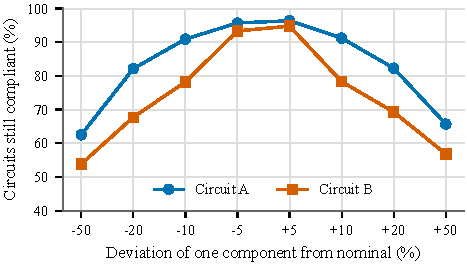
\includegraphics[width=\columnwidth]{compliance_by_magnitude}
\caption{Circuits that still meet every specification when one passive component deviates from
nominal by the given percentage. Mean over all passive components, 200 cases each.}
\label{fig:compliance}
\end{figure}

The electrode changes what the self-test sees. The gain that a healthy \cA\ measures through
$V_\mathrm{cal}$ at \SI{10}{\hertz}, relative to nominal, lies between 0.90 and 1.02 with gel and
solid-metal electrodes, between 0.59 and 1.00 with the polymer, and between 0.05 and 0.97 with
the fabrics, whose megaohm-level impedance forms a divider with the input network. The circuit
is nonetheless compliant, since the standard tests the input impedance with
\SI{620}{\kilo\ohm}.

\begin{table}[!t]
\caption{Testability of the Main Feature Set (Univariate Criterion)}
\label{tab:testability}
\centering
\setlength{\tabcolsep}{3pt}
\begin{tabular}{@{}p{0.50\columnwidth}cccc@{}}
\toprule
 & \multicolumn{2}{c}{\cA} & \multicolumn{2}{c}{\cB} \\
\cmidrule(lr){2-3}\cmidrule(l){4-5}
Electrodes & All & No porous & All & No porous \\
\midrule
Non-compliant conditions$^{\mathrm{a}}$ indistinguishable from healthy & 9 & 1 & 16 & 6 \\
Non-compliant conditions$^{\mathrm{a}}$ missed by the limit test & 15 & 3 & 35 & 8 \\
Testability rank (\SI{10}{\percent} deviation) & 2 & 4 & 2 & 3 \\
Components located without ambiguity & 4/23 & 5/23 & 2/29 & 5/29 \\
Mean number of components each one can be mistaken for & 3.9 & 2.5 & 8.6 & 5.2 \\
\bottomrule
\multicolumn{5}{@{}p{0.97\columnwidth}@{}}{\footnotesize $^{\mathrm{a}}$Fault conditions in
which most cases are non-compliant, out of 293 (\cA) and 307 (\cB).}
\end{tabular}
\end{table}


Table~\ref{tab:testability} summarizes the analysis of Section~\ref{sec:testability}. First,
some non-compliant faults cannot be seen. In \cA, eight of the nine invisible conditions are gain
errors of 5 to \SI{20}{\percent}, confused with the attenuation of a high-impedance electrode;
without porous electrodes only the open output resistor of the DRL stage remains. In \cB\ six
remain, all in the DRL stage. Second, few components can be located without ambiguity, and the
groups are predictable. The sensitivities~\eqref{eq:sensitivity} alone give, for \cA,
R5+R6+R11+R12 (the resistors that set the gain of the two stages), C5+R10 (high-pass filter),
R13+R14 (low-pass filter) and R15+R16 (reference divider); for \cB, one group with the nine
resistors that set the gain and three groups of two. Third, the structure depends on the
architecture: \cA\ has fewer invisible faults and each component can be mistaken for fewer
others.

\subsection{Compliance Decision}
\label{sec:res-decision}

\begin{table}[!t]
\caption{Compliance Decision From the Main Feature Set. Mean of Three Repetitions and
\SI{95}{\percent} Confidence Interval, in Percent}
\label{tab:decision}
\centering
\setlength{\tabcolsep}{3.5pt}
\begin{tabular}{@{}llcc@{}}
\toprule
Circuit & Method & Escapes & False rejects \\
\midrule
A & Limit test & 22.5 (21.4--23.6) & 20.0 (19.8--20.3) \\
 & Specification regression & 8.4 (6.7--10.2) & 1.5 (1.3--1.6) \\
 & Classifier & 7.9 (6.4--9.4) & 0.7 (0.4--1.0) \\
 & Classifier, \SI{1}{\percent} escape target & 0.9 (0.8--1.0) & 7.8 (4.8--10.8) \\
\addlinespace
B & Limit test & 35.3 (34.7--35.8) & 17.0 (16.5--17.6) \\
 & Specification regression & 11.4 (10.0--12.8) & 2.4 (1.9--2.9) \\
 & Classifier & 11.2 (10.3--12.1) & 1.2 (1.1--1.2) \\
 & Classifier, \SI{1}{\percent} escape target & 1.2 (0.6--1.7) & 54.0 (48.0--60.0) \\
\addlinespace
\multicolumn{4}{@{}l}{\emph{Without porous dry electrodes}} \\
A & Classifier & 4.2 (3.5--4.9) & 0.7 (0.4--0.9) \\
 & Classifier, \SI{1}{\percent} escape target & 1.0 (0.9--1.1) & 1.9 (1.3--2.5) \\
B & Classifier & 6.7 (6.2--7.1) & 1.0 (0.6--1.4) \\
 & Classifier, \SI{1}{\percent} escape target & 1.0 (0.7--1.3) & 48.7 (39.4--58.1) \\
\bottomrule
\end{tabular}
\end{table}


\begin{figure}[!t]
\centering
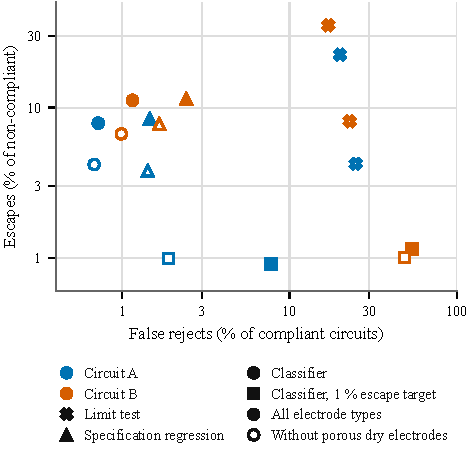
\includegraphics[width=\columnwidth]{operating_points}
\caption{Operating points of the four decision methods on the 26 features. Both axes are
logarithmic; confidence intervals are in Table~\ref{tab:decision}.}
\label{fig:operating}
\end{figure}

Table~\ref{tab:decision} and Fig.~\ref{fig:operating} give the result. The limit test accepts
between a fifth and a third of the non-compliant circuits and rejects a fifth of the compliant
ones: a wide healthy envelope, widened further by the electrodes, and a narrow compliance region
do not coincide. The specification regression and the classifier are close to each other at
their default operating points; the root-mean-square error of the predicted specifications is
between 8 and \SI{36}{\percent} of the limit, the largest for the input-impedance test.

An instrument needs a low escape rate. Lowering the threshold of the classifier brings escapes
on \cA\ to \SI{0.9}{\percent} at \SI{7.8}{\percent} of false rejects, and at only
\SI{1.9}{\percent} without porous electrodes. On \cB\ the same escape rate costs half of the
compliant circuits: the escapes that remain are the DRL faults that the measurements do not see,
as the testability analysis anticipated, and no threshold recovers a fault that leaves no trace.
A guard band on the regression is not a usable operating point (more than \SI{90}{\percent} of
false rejects at the same target). Telling the classifier which electrode type is connected does
not help (\SI{8.3}{\percent} of false rejects on \cA): the variation that matters is between
subjects, not between materials. No single measurement set suffices; with the escape target the
pulse response alone gives \SI{44}{\percent} of false rejects on \cA\ and every other set more
than \SI{75}{\percent}.

\subsection{Functional Against Percentage Severity}
\label{sec:res-severity}

A detector trained to recognize that a component is out of tolerance, scored against compliance,
rejects \SI{36.8}{\percent} of the compliant circuits of \cA\ and \SI{36.5}{\percent} of \cB,
with 7.9 and \SI{8.3}{\percent} of escapes. Trained on compliance, the same model rejects 1.6
and \SI{2.2}{\percent}, with 4.1 and \SI{7.6}{\percent} of escapes. The false rejects of the
percentage-trained detector are dominated by parametric faults that are real but harmless. (The
escapes of the functional detector are lower than in Table~\ref{tab:decision} because this
experiment weights the classes, which moves the operating point.)

\subsection{Location and Origin}
\label{sec:res-location}

There are \num{13364} non-compliant cases of \cA\ over 23 components and \num{20033} of \cB\ over
29. At the level of the a priori groups the best models reach a macro F1 of 0.87 on \cA\
(gradient boosting) and 0.76 on \cB\ (random forest), and the true group is among the three most
probable in more than \SI{99}{\percent} of the cases. At component level the macro F1 falls to
0.74 and 0.61, and the errors concentrate in the predicted groups: in \cA\ the recall is 36 to
\SI{41}{\percent} for the halves of the gain resistor and for the low-pass resistors, against 88
to \SI{100}{\percent} for most components outside a group. The recall of a component decreases
with the number of components that the testability analysis predicted it could be mistaken for
(Spearman $\rho=-0.42$, $p=0.045$ for \cA; $\rho=-0.51$, $p=0.005$ for \cB). A convolutional
network on the raw pulse response stays below the tabular models (0.56 and 0.32).

For origin, the macro F1 is 0.89 on \cA\ and 0.87 on \cB. A case with nothing to act on is
recognized in \SI{99}{\percent} of the cases and a non-compliant circuit in 94 and
\SI{92}{\percent}; circuit faults are almost never taken for electrode problems. Electrode
problems are recognized in only 64 and \SI{61}{\percent} of the cases. An open protection
resistor is always recognized and a detached electrode in 75 and \SI{89}{\percent} of the cases,
but a degraded contact only in half of the cases in \cA\ and \SI{41}{\percent} in \cB: a contact
impedance five or twenty times higher than normal for one subject falls within what healthy
contacts show on other subjects. Without porous electrodes the recall of the electrode class
rises to 76 and \SI{74}{\percent}.

\subsection{Robustness}
\label{sec:res-robustness}

\begin{figure}[!t]
\centering
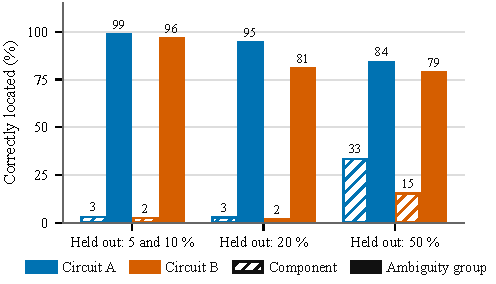
\includegraphics[width=\columnwidth]{unseen_magnitudes}
\caption{Location of the cause for parametric faults whose magnitudes were held out of training.
The model names the component; the group bars count a prediction as correct when it falls in the
ambiguity group of the true component.}
\label{fig:unseen}
\end{figure}

The compliance decision generalizes to fault magnitudes absent from training: its balanced
accuracy falls by less than 2 points with respect to a model trained with every magnitude,
except for \SI{50}{\percent} deviations on \cA\ (6 points). Component-level location does not
(Fig.~\ref{fig:unseen}): correctly located components fall from between 21 and \SI{70}{\percent}
when the magnitude was in training to between 2 and \SI{33}{\percent}. Within a group of
components with parallel sensitivities the model can only tell the members apart by the size of
the effect, that is, by memorizing the magnitudes it was shown. Counted at group level, the same
predictions remain correct in 84 to \SI{99}{\percent} of the cases on \cA\ and 79 to
\SI{96}{\percent} on \cB.

When the models are trained at the noise level and resolution at which they are used, results
barely change from 0.1 to \SI{10}{\milli\volt} of noise and from 8 to 16 bits. Trained at
\SI{1}{\milli\volt} and used at \SI{10}{\milli\volt}, escapes on \cA\ rise from 4 to
\SI{10}{\percent} and false rejects on \cB\ from 2 to \SI{19}{\percent}. A truncated Gaussian
tolerance distribution changes nothing; \SI{2}{\percent} resistors and \SI{10}{\percent}
capacitors raise escapes from 4.1 to \SI{7.1}{\percent} on \cA\ and from 7.6 to
\SI{11.4}{\percent} on \cB, and leave group-level location unchanged on \cA\ (F1 0.87) but not on
\cB\ (0.45). Raising the common-mode tone from 0.1 to \SI{1}{\volt}, or making it ten times
longer, does not make the DRL faults detectable: about half of them escape whatever the setting.
The limitation is not one of signal-to-noise ratio.

\subsection{Minimal Set of Measurements}
\label{sec:res-minimal}

\begin{figure}[!t]
\centering
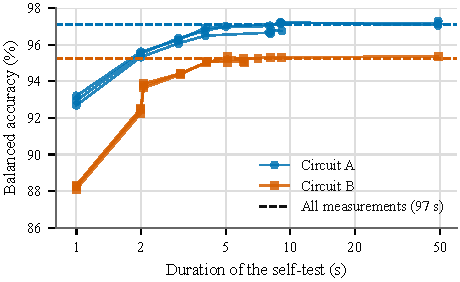
\includegraphics[width=\columnwidth]{cost_performance}
\caption{Balanced accuracy of the compliance decision on the test part as self-test measurements
are added one at a time by greedy selection on the validation part. One line per repetition.}
\label{fig:cost}
\end{figure}

The calibration pulse is always selected first (Fig.~\ref{fig:cost}). For the decision on \cA,
three measurements taking \SI{3}{\second} (the pulse, one lead-off tone and the differential tone
at \SI{150}{\hertz}) are within one point of the complete self-test of \SI{97}{\second}, in the
three repetitions. \cB\ needs a fourth, a dc reading of the DRL output, which is the measurement
that sees its DRL faults. For location on \cA, the pulse, the \SI{150}{\hertz} tone and the dc
reading of the instrumentation-amplifier output (\SI{2}{\second}) suffice in two of the three
repetitions; \cB\ needs five or six measurements. The \SI{0.05}{\hertz} tones, 80 of the
\SI{97}{\second}, are never among the first three selected.

Tables and figures for the experiments summarized in this section are in the supplementary
material.

\section{Discussion}
\label{sec:discussion}

The results support a self-test in two levels for the realistic circuit. The compliance decision
can be set to let through about \SI{1}{\percent} of the non-compliant circuits while rejecting
\SI{8}{\percent} of the compliant ones, or \SI{2}{\percent} when porous dry electrodes are
excluded. A limit test cannot approach this, because it asks whether the circuit looks like a
healthy one, which is neither necessary nor sufficient for compliance. The second level should
report an ambiguity group, not a component: the groups are known from the nominal circuit, they
hold for fault magnitudes the model has not seen, and in \cA\ a group names two to four parts
that set the same quantity. The comparison of labels has a direct practical reading: a detector
trained in the usual way of the diagnosis literature would take out of service more than a third
of the instruments that still meet the standard. The cost is low: three measurements and three
seconds give the decision, and the tones below the high-pass corner are not needed, which
matters because the self-test runs with the patient connected.

The electrode limits both levels. A healthy circuit on a high-impedance electrode measures a
reduced gain through the calibration source, which is what a gain fault looks like; on \cA\ this
accounts for eight of the nine invisible fault conditions, and false rejects fall from 7.8 to
\SI{1.9}{\percent} without porous electrodes. A
degraded contact can only be recognized against the normal contact of the same subject, which a
single self-test does not know. A self-test that kept a reference per patient, or that could
disconnect the electrodes from the calibration path, would remove most of the difficulty;
neither was studied.

The two circuits differ only in how the instrumentation amplifier is built, and that changes the
conclusions. The discrete amplifier adds seven resistors that all act on the gain and several
DRL faults that are non-compliant and invisible; evaluated only on it, the method would have been
judged unable to reach a low escape rate. This supports the argument of~\cite{chen2025} that the
circuit conditions the conclusions, with a different remedy: the ambiguity of the given circuit
is computed and the diagnosis reported at that level. The invisible DRL faults also show a limit
of the measurements: where a spare converter channel is available, a dc reading of the DRL output
is worth more than a larger common-mode tone.

\emph{Limitations.} The study is based on simulation, with behavioral amplifier models and ideal
self-test sources; transfer to hardware has not been tested. Faults are single and aging is not
modeled. The dry-electrode model rests on six subjects per material, and the gel model and the
spread between electrodes are assumed. The noise specification is computed from the rms value
and the input range from the operating point. The specifications are those of performance: some
hard faults leave the circuit compliant while removing a protection (a short across the resistor
that limits the current into the right-leg electrode), and a self-test aimed at safety would
have to label them separately.

\section{Conclusion}
\label{sec:conclusion}

An ECG front-end built around an integrated instrumentation amplifier can decide in service, from
26 features it measures on itself, whether it still complies with IEC~60601-2-25, with
\SI{0.9}{\percent} of escapes at \SI{7.8}{\percent} of false rejects; three measurements taking
three seconds come within one point of the balanced accuracy of the complete self-test. Defining
a fault by its effect on the specifications, as alternate test does, instead of by the deviation
of a component reduces false rejects from \SI{37}{\percent} to about \SI{2}{\percent}. The cause
is located with a macro F1 of 0.87 when the answer is an ambiguity group obtained from the
sensitivities of the nominal circuit, and that answer, unlike the component, remains valid for
fault magnitudes absent from training. Non-compliant circuits are separated from electrode
problems; degraded contacts are not, because they fall within the variation between subjects. A
discrete three-op-amp front-end gives a worse picture, so conclusions drawn on benchmark-like
circuits do not carry over to the circuits used in instruments. The next step is validation on
hardware; multiple faults and a per-patient reference for the electrode contact are left for
future work.


\section*{Data and Code Availability}
The simulation pipeline, the experiments and the scripts that produce every table and figure of
this paper are available at \url{https://github.com/telmomm/ecg-frontend-fault-diagnosis}. The
dataset (both circuits, with the specification values, the three levels of labels and the
configuration needed to regenerate it) is archived on Zenodo, doi:
\url{10.5281/zenodo.23134950}.

\section*{Acknowledgment}

This work uses AI-generated content. Claude (Anthropic; Claude Opus) was used to assist in
writing the code of the simulation pipeline and of the experiments, in producing the figures,
and in drafting the text of all the sections of this article. The author has reviewed and edited
the content and takes full responsibility for the final content of the paper.

\bibliographystyle{IEEEtran}
\bibliography{IEEEabrv,references}

\begin{IEEEbiographynophoto}{Telmo Miguel-Medina}
is an Associate Professor of Electronics with the Electromechanical Engineering Department,
University of Burgos, Burgos, Spain, where he teaches electronics in the health engineering and
industrial electronics degrees. He is the author of a textbook on electronics for biomedical
engineering. His research interests include biomedical electronic instrumentation, RF measurement
and electronic systems, interpretable machine learning for clinical prediction, and open and
reproducible research software.
\end{IEEEbiographynophoto}

\end{document}
